%~~~~~~~~ Chapter ~~~~~~~~
\chapter{Graphene}
\label{ch:graphene}

Graphene is one of the most studied materials in history\cite{KatsnelsonBook, Geim2007, Murakami2009, CastroNeto2009a,
Mas-Balleste2011, Konschuh2011a, Cooper2012, Han2014, Sadurni2014, Rozhkov2016}.
Even before its experimental discovery\cite{Novoselov2004, Novoselov2005},
extensive research was devoted to it\cite{Wallace1947, VanBommel1975, Semenoff1984, Haldane1988, Forbeaux1998, Oshima2000}.
All the basic properties have been discussed profusely, yet, for the sake of completeness I will make a brief recap of all the properties relevant for the rest of this thesis.\\

Graphene consists of a two-dimensional array of carbon, $C$, atoms arranged in a honeycomb lattice like the one shown in Fig.~\ref{graphene_structure}~($a-d)$)\cite{Huang2011}, an actual \ac{stm} image is also shown in $f)$. The honeycomb lattice is not a Bravais lattice itself so, in order to describe such a system in terms of Bloch functions, we have to choose a unit cell and lattice vectors to tessellate the space. Naturally there are infinite possibilities to do so, some of which are depicted in Fig.~\ref{graphene_structure}~($a-d$).
%~~~~~~~~~~~~~~~~~~~~~~~~~~ FIGURE ~~~~~~~~~~~~~~~~~~~~~~~~~%
\begin{figure}[h!]
\centering
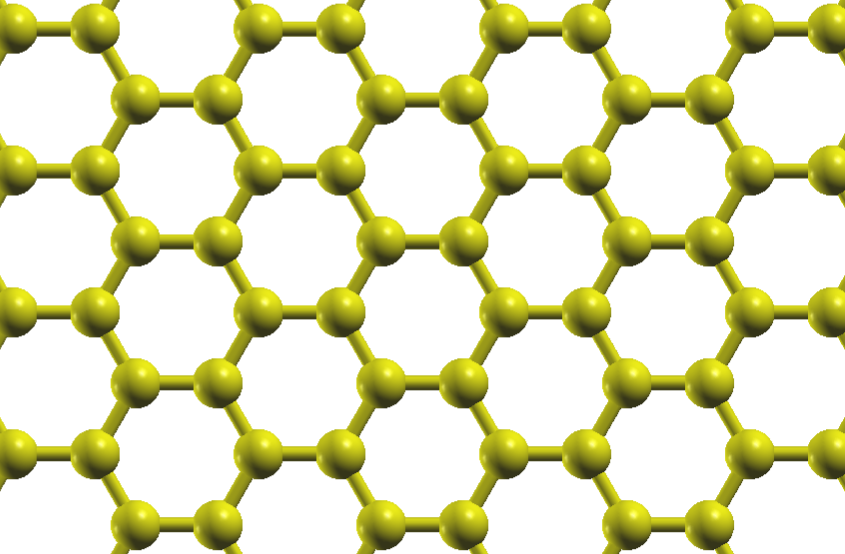
\includegraphics[width=\textwidth]{chapter04/figures/graphene.pdf}
\vspace{-7pt}
\caption{$a-d)$ Graphene atomic structure considering different unit cells and lattice vectors. Notice that, while most of the Bravais lattices are triangular, graphene can also by described with a rectangular lattice. The colored regions are the different Wigner-Seitz cells. $e)$ relevant hydrogenoid orbitals for the $C$ atom. $f)$ STM image of graphene taken from ref~\cite{Huang2011}}
\label{graphene_structure}
\end{figure}
\FloatBarrier
%~~~~~~~~~~~~~~~~~~~~~~~~~~~~~~~~~~~~~~~~~~~~~~~~~~~~~~~~~~~%
Unless otherwise stated, we will consider that the unstrained atomic distance between carbon atoms is $d_{C-C}=a=\SI{1.4}{\angstrom}$ in accordance with literature\cite{KatsnelsonBook, Cooper2012, Ishigami2007}. % TODO more biblio
The simplest unit cell and  Bravais lattice with which we can describe graphene is the one depicted in Fig.~\ref{graphene_structure}~$a)$. It consists of two atoms in the positions
\begin{equation}
\vec{r}_0 = \tfrac{a}{2}(-1,0,0) \quad;\quad
\vec{r}_1 = \tfrac{a}{2}(1,0,0),
\label{at_pos}
\end{equation}
The lattice vectors that define the triangular Bravais lattice are:
\begin{equation}
\vec{a}_1 = \tfrac{a}{2}\left(3,\sqrt{3},0\right) \quad;\quad
\vec{a}_2 = \tfrac{a}{2}\left(3,-\sqrt{3},0\right)
\label{latt_vec}
\end{equation}

Once the lattice structure is clear, we turn to the electronic properties. Carbon atoms have 6 \acp{el} allocated in five orbitals. The first two \acp{el} are in the $1s$ level, two more in the $2s$ level and finally another two \acp{el} in the $2p$ levels (Fig.~\ref{graphene_structure}~$e)$).

Since the orbitals $n=1$ are doubly occupied and far down in energy, there is no need to consider them. The $2s$ level is also full, but not so far from the Fermi energy (around $\SI{-8}{\eV}$), so we will take a look at its importance. The $2p$ orbitals are the closest to the Fermi level, hence they will play a major role in the chemistry of graphene.\\

We are going to use a \ac{tb} approximation with a basis of localized hydrogenoid orbitals. Depending on the physical property that we are interested in we will consider one of two possible basis.
One, considering only one orbital per lattice site:
\begin{equation}
  \mathcal{B}_1 = \left\{\ket{\phi^1_{p_z}}, \ket{\phi^2_{p_z}},\dots, \ket{\phi^n_{p_z}}\right\}
\label{basis1}
\end{equation}
and the other with four orbitals per atom.
\begin{equation}
  \mathcal{B}_4 = \left\{
  \ket{\phi^1_{s}},\ket{\phi^1_{p_x}},\ket{\phi^1_{p_y}},\ket{\phi^1_{p_z}},
  \dots,
  \ket{\phi^n_{s}},\ket{\phi^n_{p_x}},\ket{\phi^n_{p_y}},\ket{\phi^n_{p_z}}
  \right\}
\label{basis4}
\end{equation}
The superscript points out the atom and the subscript shows the corresponding orbital.
% These two basis describe graphene with only one orbital per site, or with four orbitals per site. The reasons why these two descriptions can be used will be shown in the following section %TODO add link



\section{Slater-Koster tight-binding model}
\label{ssec:SK}
Generally the hopping parameters are an input in any \ac{tb} model, and usually they are calculated by fitting eigenvalues (and possibly eigenfunctions) obtained from \ac{dft} calculations (the eigenfunctions are often projected to a basis of localized atomic orbitals so the interpretation in terms of hydrogenoid orbitals is easier) or by fitting experimental data to reproduce gaps, orbital components or other relevant physical properties.

As a system grows complex, more and more parameters are needed to describe it. In fact, the number of hoppings grows with the size of the basis, $n_\mathcal{B}$, as $\sum^{n_\mathcal{B}}_i i$. Nevertheless since the number of different orbitals is finite and a larger basis means only a more complex arrangement of orbitals, one could expect that not every parameter is completely independent from the others.

The \ac{sk} approximation\cite{Slater1954} takes into account the symmetry of the atomic orbitals to reduce the number of parameters needed since some of them are related by rotations or other symmetry operations.
This idea is depicted in Fig.~\ref{complex} where we can see that the hoppings $t_{p_{z},p_{x}}$ and $t_{p_{z},p_{y}}$ are in fact equivalent since one can be obtained as a rotation of the other.
%~~~~~~~~~~~~~~~~~~~~~~~~~~ FIGURE ~~~~~~~~~~~~~~~~~~~~~~~~~%
\begin{figure}[h!]
  \centering
  \includegraphics{chapter04/figures/complex.png}
  \vspace{-5pt}
  \caption{Relation between $t_{p_{z},p_{x}}$ and $t_{p_{z},p_{y}}$ hopping. In this case we need not only to rotate each orbital but also the position of the atoms, but it is clear that one hopping can be calculated as a $\pi/2$ clockwise rotation along the Z axis of the other.}
\label{complex}
\end{figure}
\FloatBarrier
%~~~~~~~~~~~~~~~~~~~~~~~~~~~~~~~~~~~~~~~~~~~~~~~~~~~~~~~~~~~%
If we define the unitary vector $\hat{r} = \vec{r}/|\vec{r}|$ and its components $\hat{r}=(l,m,n)$ we can see that
\begin{equation}
  t_{p_{z},p_{x}} (l,m,n) = t_{p_{z},p_{y}}(m,l,n)
\end{equation}
notice that the change in the arguments is equivalent to perform a rotation of the vector $\vec{r}$ of $-\pi/2$ around the $Z$ axis.


Even though this transformations can be deduced by sheer ``brute force'', there is a more general approach that allows the decomposition of any arbitrary hopping in a finite set of bond types.

The easiest way to visualize this decomposition is to consider the hopping between any two orbitals by an arbitrary vector $\vec{r}$, as depicted in the right panel of Fig.~\ref{bonds}. % TODO add letter to panels
Such a hopping can be decomposed in two contributions depending on the relative orientation of the orbitals, namely $\pi$-bonds and $\sigma$-bonds (see Fig.~\ref{bonds}).
%~~~~~~~~~~~~~~~~~~~~~~~~~~ FIGURE ~~~~~~~~~~~~~~~~~~~~~~~~~%
\begin{figure}[h!]
\centering
\includegraphics{chapter04/figures/bonds.png}
\vspace{-5pt}
\caption{$a)$ Only two different types of bonds between $p$ orbitals. $b)$ Simplification of the \ac{sk} hopping parameter by decomposing the hopping into its $\sigma$ and $\pi$ component, in this case it is easy to see that the hopping from any $p_{z}$ orbital to another one that in the $XY$ plane will be purely a $\pi$ bond.}
\label{bonds}
\end{figure}
\FloatBarrier
%~~~~~~~~~~~~~~~~~~~~~~~~~~~~~~~~~~~~~~~~~~~~~~~~~~~~~~~~~~~%
% TODO somewhere else? % We can notice in Fig.~\ref{bonds} that in the case of pristine graphene all the in-plane $p_z$-$p_z$ hoppings will be purely $\pi$ bonds, while the other $s$-$p$ hoppings will be $\sigma$ bonds.\\
The $p_z$-$p_z$ hopping for two orbitals separated by a vector $\vec{r}=|\vec{r}|(l,m,n)$ can be calculated as:
\begin{equation*}
 t_{p_z-p_z} = n^2V_{pp\sigma} + (1-n^2)V_{pp\pi}
\end{equation*}
as it follows, if both orbitals lie in the $XY$ plane, then $n=0$ so the hopping will be a purely $\pi$ bond. However, if the orbitals are placed along the $Z$ axis ($n=1$) the bond would be a $\sigma$ bond.

Any hopping between orbitals can be decomposed into its components ($\sigma/\pi$ for $p$ orbitals) requiring only 3 parameters: $V_{ss\sigma}$, $V_{sp\sigma}$, $V_{sp\pi}$ to describe all 10 hoppings among $s$ and $p$ orbitals.


Another nice feature of the \ac{sk} approximation is that the atomic distances are encoded in the magnitude of the \ac{sk} parameters and the coefficients ($l$, $m$, $n$) in the analytic formulas (see \ref{SKhoppings}) are the responsible for capturing the symmetries arising both form the orbitals and the lattice structure.\\

%XXX Add SK formulas?

This decoupling of distance and direction in the hoppings provides a simple model able to capture the effects of geometric deformations, strain and symmetry (breaking) in the atomic structure.


As an example of the capabilities of the \ac{sk} model, we show its versatility by computing the band structure and \ac{dos} of well known materials such as graphene, \ac{bn} and Bismuth.

%
% Graphene TB
%
The \ac{sk} parameters, in $\si{\eV}$, used for graphene are:
\begin{equation}
  \begin{array}{l|cccc}
    Hopping & V_{ss\sigma} & V_{sp\sigma} & V_{pp\sigma} & V_{pp\pi} \\ \hline
    C-C & -7.76 & 8.16 & 7.48 & -2.7 \\
    C-H & -6.84 & 7.81 & \text{--} & \text{--}
  \end{array}\qquad\qquad
  \begin{array}{c|cccc}
    \text{On-site} & s & p_x & p_y & p_z \\ \hline
    C & -8.8 & 0.0 & 0.0 & 0.0 \\
    H & -2.5 &     &     &
  \end{array}
\label{G_SK_params}
\end{equation}
These values are either fitted from \ac{dft} bands or taken from \cite{}. The $C-H$ hoppings are included since they will be necessary when finite systems are considered and the edges need passivation.
The $h$-$BN$ parameters can be chosen as those of graphene with a different on-site energy for all the orbitals in the $B$ and $N$ atoms, namely $E_{B} = -E_{N} =\SI{2.5}{\eV}$.

%
% Bi TB
%
In order to describe Bismuth, we we require up to third neighbor hoppings. The \ac{sk} parameters are taken from~\citen{Liu1995}:
\begin{equation}
  \begin{array}{c|cccc}
    Hopping & V_{ss\sigma} & V_{sp\sigma} & V_{pp\sigma} & V_{pp\pi} \\ \hline
    1 & -0.608 & 1.32 & 1.854 & -0.6 \\
    2 & -0.384 & 0.433 & 1.396 & -0.344 \\
    3 & \text{--} & \text{--} & 0.156 & \text{--}
  \end{array}\qquad\qquad
  \begin{array}{c|cccc}
    \text{On-site} & s & p_x & p_y & p_z \\ \hline
    Bi & -10.906 & -0.486 & -0.486 & -0.486 \\
  \end{array}
\label{Bi_SK_params}
\end{equation}

Using these parameters in the same \ac{sk} formal model, the obtained band structure and \ac{dos} is shown in Fig.~\ref{SKbands}.

%~~~~~~~~~~~~~~~~~~~~~~~~~~ FIGURE ~~~~~~~~~~~~~~~~~~~~~~~~~%
\begin{figure}[h!]
\centering
\includegraphics{graphene/figures/banddos.pdf}
\vspace{-15pt}
\caption{Graphene bands in the \ac{sk} approximation, with $s$, $p_x$, $p_y$, $p_z$ orbitals for the $C$ atoms. The color denote the $p_z$ component of each state. It can be seen that the $p_z$ orbital are decoupled from the rest of the orbitals and at low energy they are enough to describe the system}
\label{SKbands}
\end{figure}
\FloatBarrier
%~~~~~~~~~~~~~~~~~~~~~~~~~~~~~~~~~~~~~~~~~~~~~~~~~~~~~~~~~~~%
For all panels, the color, $\mathcal{C}$ represents the weight of the $p_z$ orbital in each state:
%Figure~\ref{Gbands} show the graphene band structure along the $\Gamma,K,K',\Gamma$ path when 4 orbitals per Carbon atom are used, hence the our basis is \eqref{basis4}. In the \ac{tb} approximation any eigenstate of the Hamiltonian will be expressed as a combination of the states of the basis, the color in the band structure is proportional to the expectation value of the $p_z$ projector operator,$\mathcal{O}_{p_z}$,
\begin{equation*}
   \mathcal{C} = \bra{\psi_{\alpha}}\mathcal{O}_{p_z}\ket{\psi_{\alpha}}
\end{equation*}
where $\mathcal{O}_{p_z}$ is the $p_z$ projector operator and
\begin{equation*}
  H\ket{\psi_{\alpha}} = E_{\alpha}\ket{\psi_{\alpha}} \qquad ; \qquad
   \ket{\psi} = \sum_i c_i\ket{\phi_i} \quad
   \text{for} \quad\ket{\phi_i}\in\mathcal{B}_4
\end{equation*}

\section{Basic Properties}
\label{sec:graphene_basic_properties}
We are going to start by using the four orbital basis \eqref{basis4} with the geometry of Fig.~\ref{graphene_structure}~$a)$. Our Hamiltonian will have two atoms per unit cell and four orbitals per atom, so it will be a $8\times8$ matrix\footnote{we consider now spinless fermions.}.

In order to calculate the Hamiltonian matrix we need the ten different hoppings that describe the hopping between every pair of orbitals: $t_{s-s}$, $t_{s-p_x}$, $t_{s-p_y}$, ... Nevertheless, the number of parameters necessary can be reduced using the symmetries of the orbitals as shown in the next subsection.



\subsection{Bands}



\subsection{Low energy regime}
Notice that the bands close to the Fermi Energy ($E=0$) only have $p_z$ component, this is due to the mirror symmetry of the $p_z$ orbital and the atomic structure of graphene (planar). In fact this decoupling from the rest of the orbitals allows the
Even in the presence of some interactions that, indeed, mix the $p_z$ manifold with other orbitals, the $p_z$ is still the main component of the low energy spectra.

An example of such a situation is the graphene bilayer, which be studied in detail in chapter~\ref{ch:bilayer}. In this system the $p_z$ and $s$ orbitals of different layers have a finite hopping, nevertheless when we plot the bands %TODO figure of Gbilayer
we see that most of the contribution is still $p_z$ ($>98\%$ for realistic values of the hoppings).







\section{Physical properties of Graphene}
The \ac{sk} parameters, in $\si{\eV}$, used for graphene are:
\begin{equation}
  \begin{array}{l|cccc}
    Hopping & V_{ss\sigma} & V_{sp\sigma} & V_{pp\sigma} & V_{pp\pi} \\ \hline
    C-C & -7.76 & 8.16 & 7.48 & -2.7 \\
    C-H & -6.84 & 7.81 & \text{--} & \text{--}
  \end{array}\qquad\qquad
  \begin{array}{c|cccc}
    \text{On-site} & s & p_x & p_y & p_z \\ \hline
    C & -8.8 & 0.0 & 0.0 & 0.0 \\
    H & -2.5 &     &     &
  \end{array}
\label{SK_params}
\end{equation}





%The \ac{sk} parameters used for graphene are:
%\begin{equation}
%  V_{ss\sigma}= \SI{-7.76}{\eV} \quad;\quad
%  V_{sp\sigma}= \SI{8.16}{\eV} \quad;\quad
%  V_{pp\sigma}= \SI{7.48}{\eV} \quad;\quad
%  V_{pp\pi}= \SI{-2.7}{\eV}
%\label{sk_params}
%\end{equation}



%\input{graphene/qsh.tex}
